\documentclass[12pt]{article}
\usepackage[utf8]{inputenc}
\usepackage{listings}
\usepackage{xcolor}
\usepackage{graphicx}
\usepackage{amsmath}

\definecolor{codegreen}{rgb}{0,0.6,0}
\definecolor{codegray}{rgb}{0.5,0.5,0.5}
\definecolor{codepurple}{rgb}{0.58,0,0.82}
\definecolor{backcolour}{rgb}{0.95,0.95,0.92}
\lstdefinestyle{mystyle}{
    backgroundcolor=\color{backcolour},   
    commentstyle=\color{codegreen},
    keywordstyle=\color{magenta},
    numberstyle=\tiny\color{codegray},
    stringstyle=\color{codepurple},
    basicstyle=\ttfamily\footnotesize,
    breakatwhitespace=false,         
    breaklines=true,                 
    captionpos=b,                    
    keepspaces=true,                 
    numbers=left,                    
    numbersep=5pt,                  
    showspaces=false,                
    showstringspaces=false,
    showtabs=false,                  
    tabsize=2
}

\lstset{style=mystyle}
\begin{document}
\title{CSDS 391 Programming Assignment 2 Writeup}
\author{Ningjia Huang, Tianxi Zhao}
\date{Due On: December 4, 2020}
\maketitle

\section*{Problem 1: }

\section*{Problem 2: }
\subsection*{(a)}
The mean squared error is calculated using the following equation: 
\begin{center}
    $MSE = \frac{1}{n}\sum_n (Y_i - \hat{Y_i})^2$
\end{center}
, where $Y_i$ is the actual category of the $ith$ item and $\hat{Y_i}$ is the predicted category by using our neural network.\\ \\
The following codes compute the \textbf{mean squared error} for iris data. The parameter "data\_vector" are the attributes we would like to take into account, it should be a dataframe of attributes.
$w_0, w_1, w_2$ define the weights of neural network. The parameter "pattern\_classes" is a dataframe of the category corresponding to the data\_vectors. The \textbf{mean\_square\_error} makes use of 
the logistic non-linearity function in Problem 1.
\begin{lstlisting}[language=Python, caption=Mean Squared Error Calculation]
# data vectors in dataframe, pattern classes in list
def mean_square_error(data_vectors, w0, w1, w2, pattern_classes):
    n = data_vectors.shape[0]
    data_vectors_list = data_vectors.values.tolist()
    pattern_classes_list = pattern_classes.tolist()
    temp_mse = 0
    for i in range(n):
        temp_mse = temp_mse + np.square(pattern_classes_list[i] - one_layer_network(w0, w1, w2, data_vectors_list[i][0], data_vectors_list[i][1]))
    mse = temp_mse/n
    return mse
\end{lstlisting}

\subsection*{(b)}
To plot the linear boundary, we find the x-intercept and y-intercept by using the following code: 
\begin{lstlisting}[language=Python, caption=Plot Mean Squared Error]
plot([0,-w0/w1],[-w0/w2,0])
\end{lstlisting}
\subsubsection*{2.b.1}
The first set of weights we've chosen is $[-3.9, 0.46, 0.95]$. The mean squared error we concluded is 0.13235245817007218. The following figure shows the linear boundary with our chosen set of weights. As we can tell from the graph, the
linear boundary generally seperates the two categories of iris. 
\begin{center}
    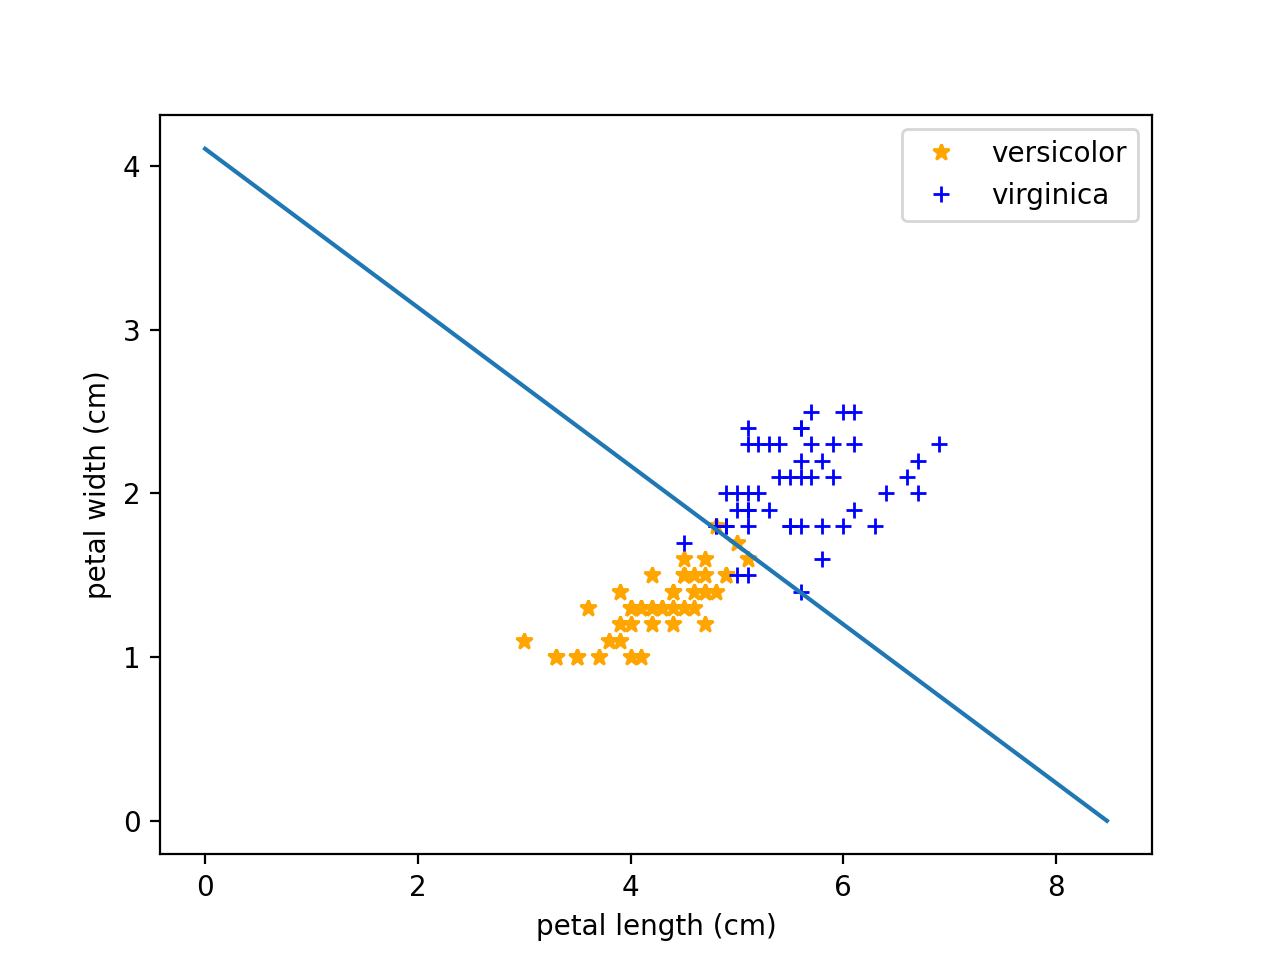
\includegraphics[scale=0.6]{fig/p2_b1.png}
\end{center}

\subsubsection*{2.b.2}
The second set of weights we've chosen is $[-1, 0.7, 2]$. The mean squared error we concluded is 0.48802189762271864. The following figure shows the linear boundary with our chosen set of weights. As we can tell from the graph, the linear boundary does not seperate these two categories 
at all. 
\begin{center}
    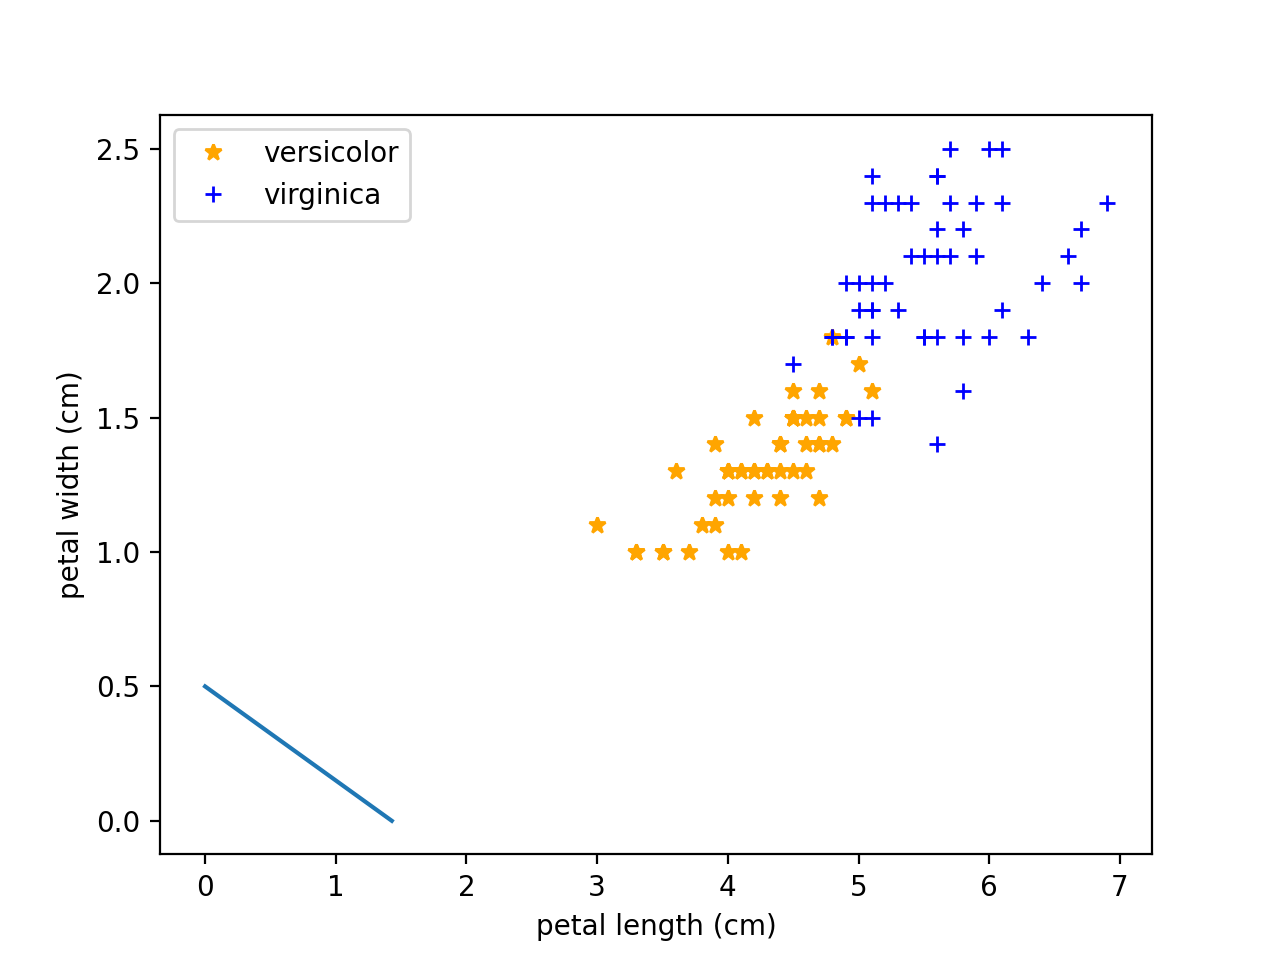
\includegraphics[scale=0.6]{fig/p2_b2.png}
\end{center}

\subsection*{(c)}
To compute the gradient of the objective function, we need to take the derivative of the objective function. Assume \textbf{x$_i$} is the ith row with attribute petal length and petal width such that $x_i = [1,x_{i1},x_{i2}]$($1$ is placed here because $w_0$ requires 1 to be its coefficient). \textbf{w} is the set of weights for the attributes. The logistic function we get is:
\begin{center}
    $\sigma(z) = \frac{1}{1+e^{-z}} = \frac{1}{1+e^{w \cdot x}}$
\end{center}
Therefore, the mean squared function becomes: 
\begin{center}
    $MSE = \frac{1}{N} \sum_{i = 1}^{n}(\sigma(w\cdot x_i)-y_i)^2$
\end{center}
By taking the derivative of this objective function with respect to $w_0$, we have: 
\begin{center}
    $\frac{\partial MSE}{\partial w_0} = \frac{2}{N}\sum_{i=1}^{N}(\sigma(w \cdot x_i)-y_i)\frac{\partial \sigma}{\partial w_0}$ \\ 
    $\frac{\partial MSE}{\partial w_0} = \frac{2}{N}\sum_{i=1}^{N}(\sigma(w \cdot x_i)-y_i)(1-\sigma(w \cdot x_i))(\sigma(w\cdot x_i))\frac{\partial (w\cdot x)}{\partial w_0}$ \\ 
    $\frac{\partial MSE}{\partial w_0} = \frac{2}{N}\sum_{i=1}^{N}(\sigma(w \cdot x_i)-y_i)(1-\sigma(w \cdot x_i))(\sigma(w\cdot x_i))$
\end{center}
Similarly, by only changing the last derivative $\frac{\partial(w\cdot x)}{\partial w_0}$ to $\frac{\partial(w\cdot x)}{\partial w_1}$ and $\frac{\partial(w\cdot x)}{\partial w_2}$, we can compute the derivative of the objective function with respect to $w_1$ and $w_2$:
\begin{center}
    $\frac{\partial MSE}{\partial w_1} = \frac{2}{N}\sum_{i=1}^{N}(\sigma(w \cdot x_i)-y_i)(1-\sigma(w \cdot x_i))(\sigma(w\cdot x_i))x_{i1}$
    $\frac{\partial MSE}{\partial w_2} = \frac{2}{N}\sum_{i=1}^{N}(\sigma(w \cdot x_i)-y_i)(1-\sigma(w \cdot x_i))(\sigma(w\cdot x_i))x_{i2}$
\end{center} 
Therefore, the gradient of MSE is: 
\begin{center}
    $\nabla MSE = \left[\begin{array}{@{}c@{}}
        \frac{\partial MSE}{\partial w_0} \\ \\
        \frac{\partial MSE}{\partial w_1} \\ \\
        \frac{\partial MSE}{\partial w_2} 
        \end{array} \right] = \left[\begin{array}{@{}c@{}}
            \frac{2}{N}\sum_{i=1}^{N}(\sigma(w \cdot x_i)-y_i)(1-\sigma(w \cdot x_i))(\sigma(w\cdot x_i)) \\ \\
            \frac{2}{N}\sum_{i=1}^{N}(\sigma(w \cdot x_i)-y_i)(1-\sigma(w \cdot x_i))(\sigma(w\cdot x_i))x_{i1} \\ \\ 
            \frac{2}{N}\sum_{i=1}^{N}(\sigma(w \cdot x_i)-y_i)(1-\sigma(w \cdot x_i))(\sigma(w\cdot x_i))x_{i2}
        \end{array} \right]$
\end{center}

\subsection*{(d)}
\subsubsection*{scalar form: }
The scalar form of the gradient is computed in Problem 2 (c): 
\begin{center}
    $\nabla MSE = \left[\begin{array}{@{}c@{}}
        \frac{\partial MSE}{\partial w_0} \\ \\
        \frac{\partial MSE}{\partial w_1} \\ \\
        \frac{\partial MSE}{\partial w_2} 
        \end{array} \right] = \left[\begin{array}{@{}c@{}}
            \frac{2}{N}\sum_{i=1}^{N}(\sigma(w \cdot x_i)-y_i)(1-\sigma(w \cdot x_i))(\sigma(w\cdot x_i)) \\ \\
            \frac{2}{N}\sum_{i=1}^{N}(\sigma(w \cdot x_i)-y_i)(1-\sigma(w \cdot x_i))(\sigma(w\cdot x_i))x_{i1} \\ \\ 
            \frac{2}{N}\sum_{i=1}^{N}(\sigma(w \cdot x_i)-y_i)(1-\sigma(w \cdot x_i))(\sigma(w\cdot x_i))x_{i2}
        \end{array} \right]$
\end{center}

\subsubsection*{vector form: }
Let $X = \left[\begin{array}{@{}c@{}}
        x_{11}, x_{12}, 1 \\
        \dots \\
        x_{n1}, x_{n2}, 1
         \end{array} \right]$, which is a matrix represents the attributes(1 corresponds for bias).
Since the term $\frac{2}{N}\sum_{i=1}^{N}(\sigma(w \cdot x_i)-y_i)(1-\sigma(w \cdot x_i))(\sigma(w\cdot x_i))$ is independent of the dimension
$j$ and common for $\frac{\partial MSE}{\partial w_0}$, $\frac{\partial MSE}{\partial w_1}$, and $\frac{\partial MSE}{\partial w_2}$, we can first express 
this term as $z_i = (\sigma(w \cdot x_i)-y_i)(1-\sigma(w \cdot x_i))(\sigma(w\cdot x_i))$. The gradient of MSE becomes: 
\begin{center}
    $\nabla MSE = \frac{2}{m} \left[\begin{array}{@{}c@{}}
                \sum_{i=1}^{N} z_i \\
                \sum_{i=1}^{N} z_{i}x_{i1} \\
                \sum_{i=1}^{N} z_{i}x_{i2}
                \end{array} \right] = \frac{2}{m}\left[\begin{array}{@{}c@{}}
                                     1, \dots, 1 \\
                                     x_{11}, \dots, x_{n1} \\
                                     x_{12}, \dots, x_{n2}
                                     \end{array} \right] \left[\begin{array}{@{}c@{}}
                                                         z_1 \\
                                                         \dots \\
                                                         z_n
                                                         \end{array}\right] = \frac{2}{m}\mathbf{X^{T}}\left[\begin{array}{@{}c@{}}
                                                            z_1 \\
                                                            \dots \\
                                                            z_n
                                                            \end{array}\right] $
\end{center}
Then, we attempt to expand the vector $z_i = \left[\begin{array}{@{}c@{}}
                                             z_1 \\
                                             \dots \\
                                             z_n
                                             \end{array} \right]$ :
\begin{center}
    $z_i = \left[\begin{array}{@{}c@{}}
            (\sigma(\mathbf{w \cdot x_1})-y_1)(1-\sigma(\mathbf{w \cdot x_1}))(\sigma(\mathbf{w\cdot x_1})) \\
            \dots \\
            (\sigma(\mathbf{w \cdot x_n})-y_n)(1-\sigma(\mathbf{w \cdot x_n}))(\sigma(\mathbf{w\cdot x_n})) 
            \end{array} \right]= \left[\begin{array}{@{}c@{}}
                                 \sigma(\mathbf{w \cdot x_1})-y_1 \\ 
                                 \dots \\
                                 \sigma(\mathbf{w \cdot x_n})-y_n
                                 \end{array} \right] \star \left[\begin{array}{@{}c@{}}
                                                           1-\sigma(\mathbf{w \cdot x_1}) \\
                                                           \dots \\
                                                           1-\sigma(\mathbf{w \cdot x_n})
                                                           \end{array} \right] \star \left[\begin{array}{@{}c@{}}
                                                                                     \sigma(\mathbf{w\cdot x_1}) \\
                                                                                     \dots \\
                                                                                     \sigma(\mathbf{w\cdot x_n})
                                                                                     \end{array} \right]$
\end{center}
The $\star$ operation is defined as multiplying the ith row's elements. To simplify the expression, let $\sigma(\mathbf{Xw}) = \left[\begin{array}{@{}c@{}}
                                                                                                         \sigma(\mathbf{w^{T}x_1}) \\
                                                                                                         \dots \\
                                                                                                         \sigma(\mathbf{w^{T}x_n})
                                                                                                         \end{array} \right]$. 
Thus, $z_i$ can be expressed as $z_i = (\sigma(\mathbf{Xw})-\mathbf{y})\star(1 - \sigma(\mathbf{Xw}))\star \sigma(\mathbf{Xw})$. The vector form of gradient can be expressed as: 
\begin{center}
    $\nabla MSE = \frac{2}{m}\mathbf{X^T}(\sigma(\mathbf{Xw})-\mathbf{y})\star (\mathbf{1} - \sigma(\mathbf{Xw}))\star \sigma(\mathbf{Xw})$
\end{center}

\subsection*{(e)}
The code we used to calculate the gradient is as following: 
\begin{lstlisting}[language=Python, caption=Calculate Gradient]
def summed_gradient(x, w0, w1, w2, y): 
    sigmoid_list = []
    n = len(x)
    error_list = []
    coefficient_list = []
    x = x.values.tolist()
    y = y.tolist()
    for i in range(len(x)): 
        sigmoid_list.append(one_layer_network(w0, w1, w2, x[i][0], x[i][1]))
        error_list.append(sigmoid_list[i] - y[i])
        coefficient_list.append(error_list[i] * sigmoid_list[i] * (1 - sigmoid_list[i]))
    # number of rows = number of rows in data vectors, number of columns = number of columns in data vector + 1 since 1 for bias coefficient
    temp_matrix = np.ones((len(x), len(x[0]) + 1))
    temp_matrix[:, 1:] = x
    sum_term = np.zeros((len(x), len(x[0]) + 1))
    for i in range(len(coefficient_list)):
        sum_term[i] = (2/n) * temp_matrix[i] * coefficient_list[i]
    return np.sum(sum_term, axis = 0)
\end{lstlisting}
Let step size = 0.01. With the input weight $[w0, w1, w2] = [-5, 0.5, 2]$, we concluded the following table for the illustration of how the decision boundary changes for a small step: 
\begin{center}
    \begin{tabular}{| c | c | c |}
        \hline
        & old data & adjusted data\\
        \hline
        weights & [-5, 0.5, 2] & [-5.00080742  0.49665344  1.9989812] \\
        \hline
        MSE & 0.48802189762271864 & 0.4879972995169846 \\
        \hline
        decision boundary & m = -0.35, b = 0.5 & m = -0.3497940478, b = 0.500093299\\
        \hline
    \end{tabular}
\end{center}
As we can tell from the table, the mean squared error reduced a little bit as we made a small step. To visualize the change of decision boundary, please refer to the following graph: 
\begin{center}
    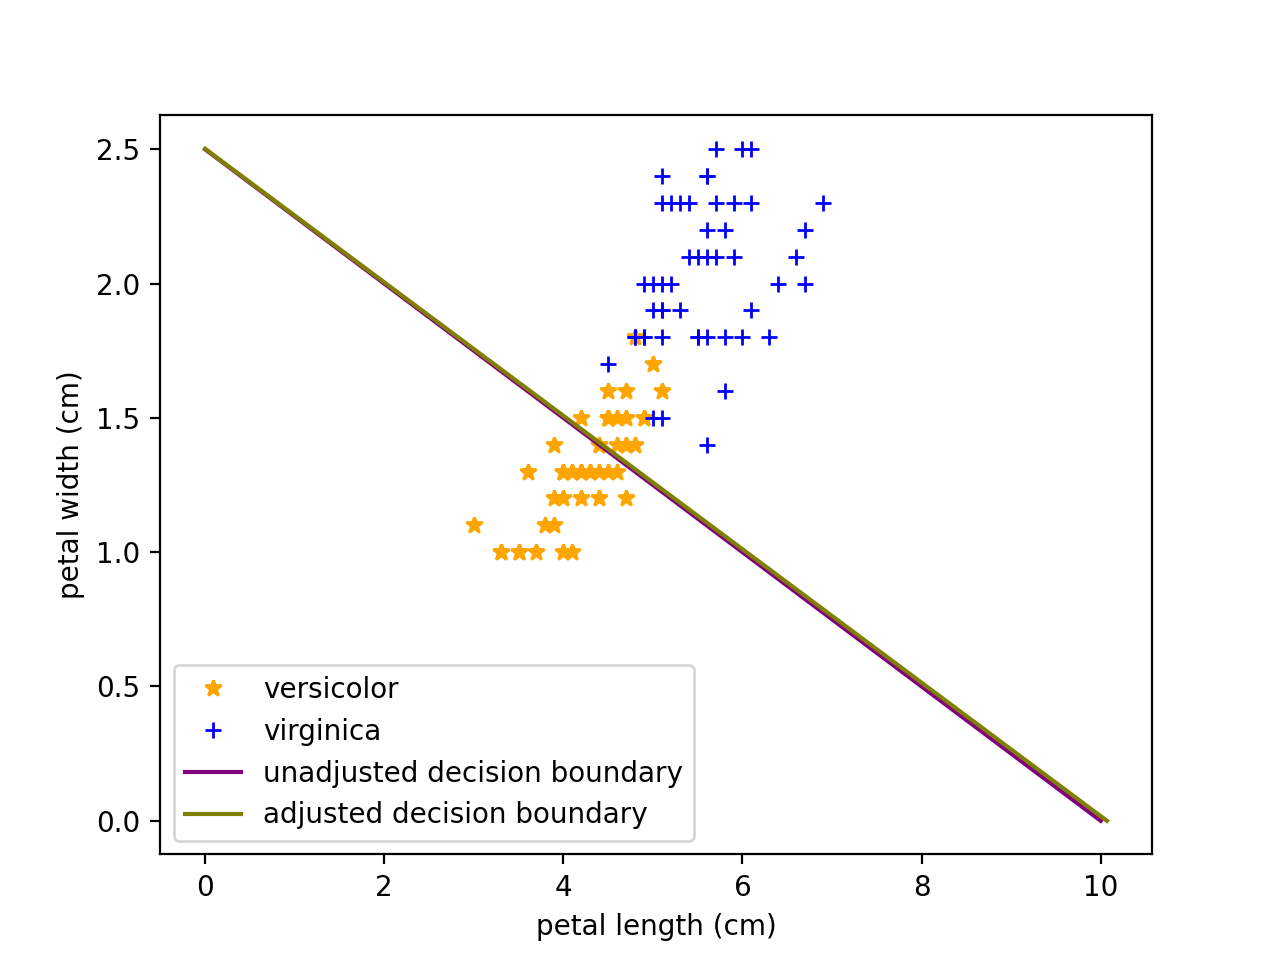
\includegraphics[scale=0.6]{fig/p2e1.png}
\end{center}
Since the small step is kind of hard to visualize, we run this process for $10000$ times in order to enlarge the difference. The following two graphs show the decision boundary before the
adjustment and after the adjustment: 
\begin{center}
    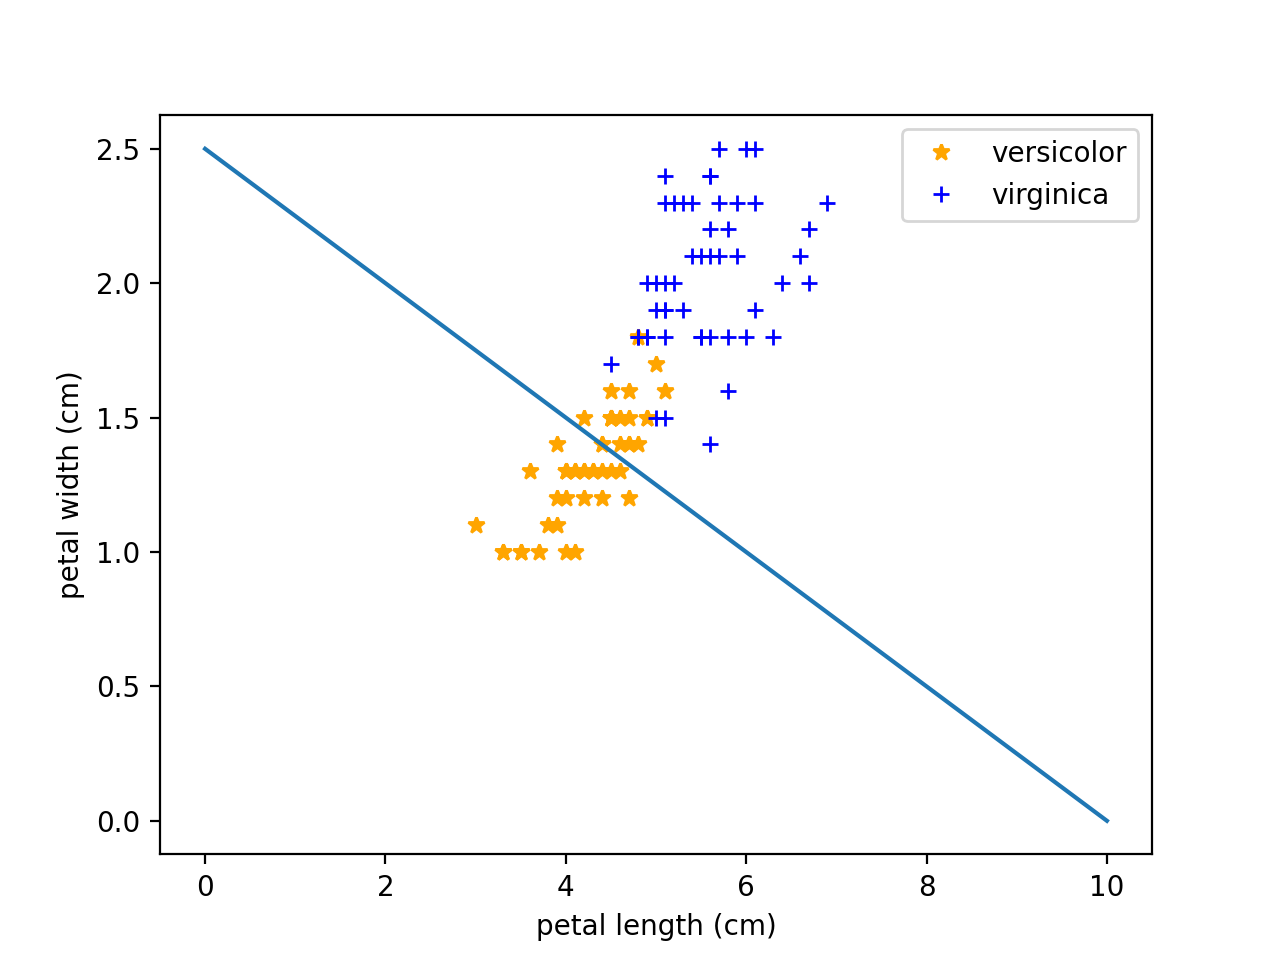
\includegraphics[scale=0.4]{fig/p2e2.png} 
    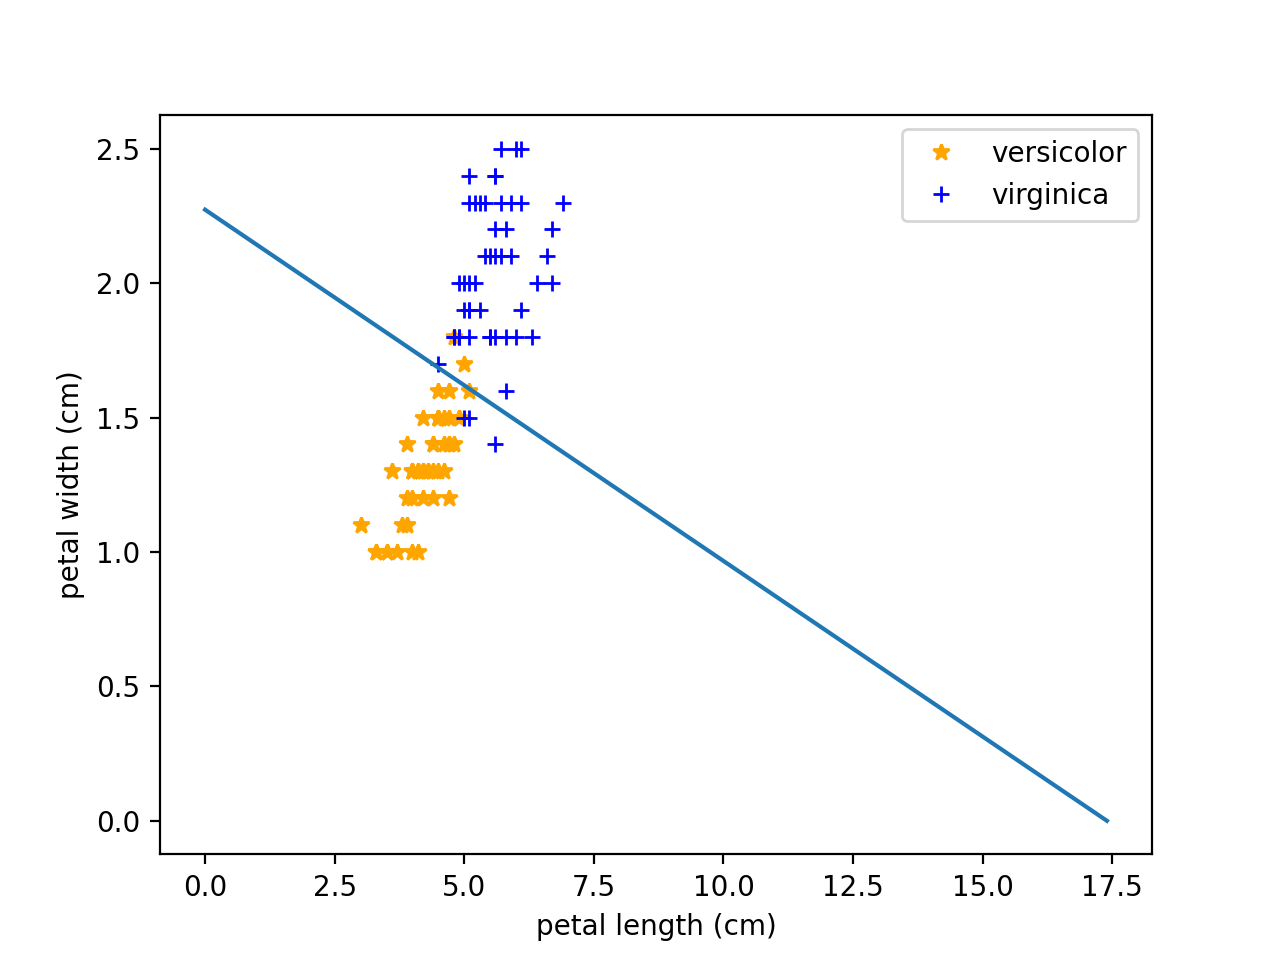
\includegraphics[scale=0.4]{fig/p2e3.png}
\end{center}
The code we used for this illustration is: 
\begin{lstlisting}[language=Python, caption=Illustration of the Change of Gradient]
def illustrate_summed_gradient(x, w0, w1, w2, y):
    num_of_iter = []
    for i in range(10000):
        num_of_iter.append(i+1)
        temp1, temp2, temp3 = summed_gradient(x, w0, w1, w2, y)
        w0 = w0 - 0.01 * temp1
        w1 = w1 - 0.01 * temp2
        w2 = w2 - 0.01 * temp3
    plot([0,-w0/w1],[-w0/w2,0])
    \end{lstlisting}
\end{document}